\section{ĐÁNH GIÁ HIỆU NĂNG VÀ KẾT LUẬN}\label{sec:danh_gia_hieu_nang}

Chương này trình bày kết quả thực nghiệm định lượng từ 5 kịch bản đo lường tự động, bao gồm: phân tích bảng số liệu Throughput, đồ thị so sánh thời gian hội tụ khi Spine Switch gặp sự cố, bảng kiểm soát các lỗ hổng bị chặn đứng bởi chính sách Micro-segmentation, và đánh giá tổng thể hiệu năng hệ thống. Toàn bộ số liệu được trích xuất trực tiếp từ bộ đếm nhân Linux (\texttt{/sys/class/net/.../statistics/tx\_bytes}), đảm bảo tính khách quan và khả năng tái lập.

\subsection{Đánh giá Thời gian Hội tụ OSPFv3}

\subsubsection{Kịch bản Giả lập Sự cố (Case 1 \& Case 2)}

Hai kịch bản được thiết kế để đo thời gian hội tụ OSPFv3 khi một Spine Switch gặp sự cố và khi khôi phục:

\begin{itemize}
    \item \textbf{Case 1 (Convergence Down):} Tại giây thứ 6, toàn bộ các liên kết của Spine S1 đến các Leaf (s1-eth1, s1-eth2, s1-eth3) bị \texttt{down} đồng loạt, mô phỏng đứt cáp quang.
    \item \textbf{Case 2 (Convergence Up):} Sau khi S1 đã sập, các liên kết được khôi phục (\texttt{ip link set up}), đo thời gian OSPFv3 cập nhật lại bảng định tuyến.
\end{itemize}

Hệ thống giám sát ghi nhận Throughput mỗi giây từ bộ đếm TX\_Bytes trên giao diện truyền dữ liệu.

\subsubsection{Đồ thị So sánh Thời gian Hội tụ}

\begin{figure}[H]
    \centering
    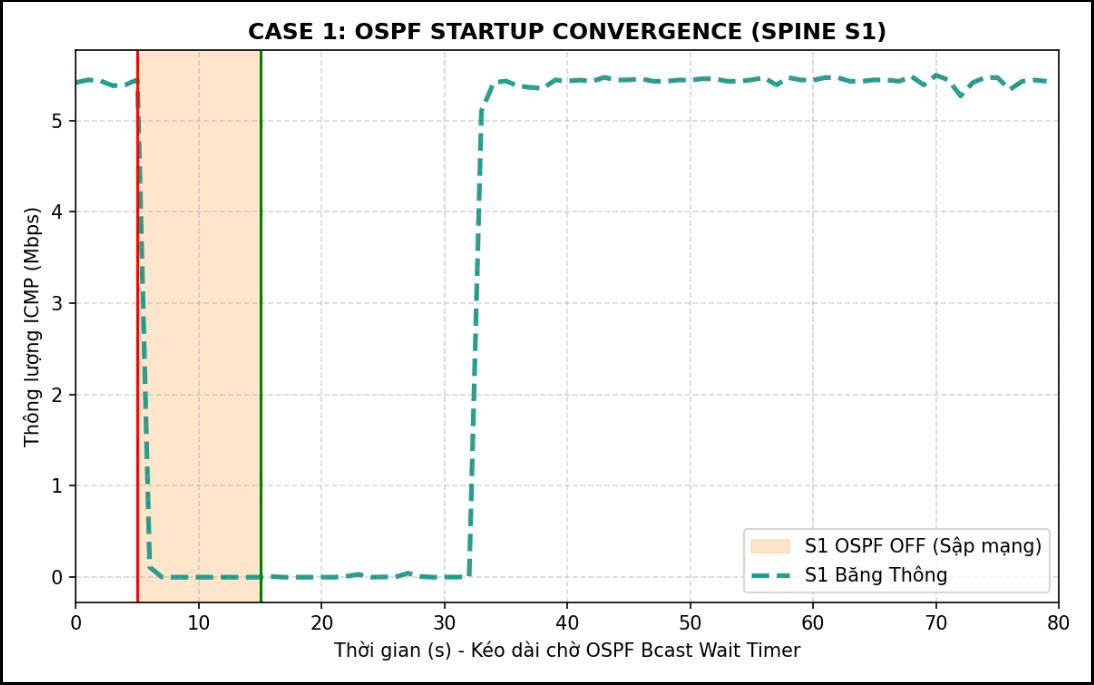
\includegraphics[width=\textwidth]{image/case1.jpg}
    \caption{Biểu đồ throughput khi sập Spine S1 — Thời gian hội tụ $\sim$27 giây (Case 1).}
    \label{fig:case1}
\end{figure}

\begin{figure}[H]
    \centering
    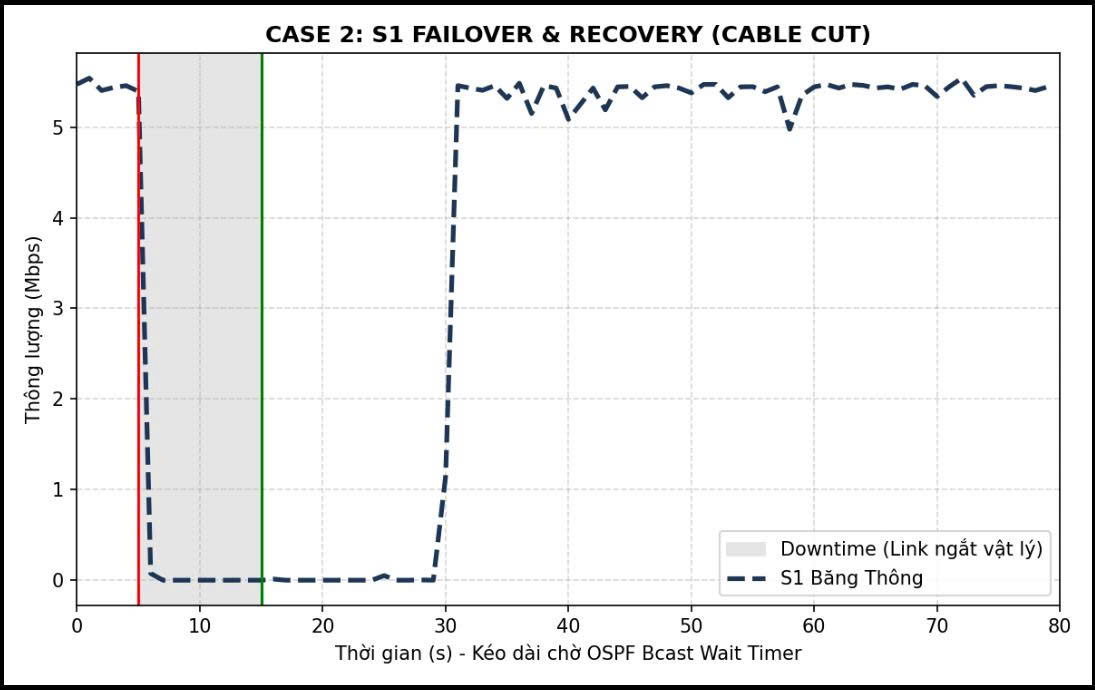
\includegraphics[width=\textwidth]{image/case2.jpg}
    \caption{Biểu đồ throughput khi khôi phục Spine S1 — Thời gian hội tụ $\sim$24 giây (Case 2).}
    \label{fig:case2}
\end{figure}

\subsubsection{Bảng Phân tích Số liệu Throughput}

Dữ liệu từ các tệp \texttt{case1.csv} (80 mẫu) và \texttt{case2.csv} (80 mẫu) cho thấy các giai đoạn rõ ràng:

\begin{table}[H]
    \centering
    \caption{Phân tích chi tiết các giai đoạn hội tụ OSPFv3 khi sập S1 (Case 1).}
    \label{tab:case1_analysis}
    \begin{tabular}{|l|l|p{7cm}|}
        \hline
        \textbf{Giai đoạn} & \textbf{Thời gian} & \textbf{Throughput và Nhận xét} \\
        \hline
        Ổn định (Trước sự cố) & t=0$\sim$5 & 5,39--5,45 Mbps. Hệ thống hoạt động bình thường. \\
        \hline
        Phát hiện sự cố & t=6 & Throughput giảm đột ngột xuống 0,111 Mbps. \\
        \hline
        Gián đoạn hoàn toàn & t=7$\sim$15 & Throughput = 0 Mbps. Mạng mất kết nối 9 giây liên tiếp. \\
        \hline
        Hội tụ từng phần & t=16$\sim$32 & Throughput dao động 0,001--0,044 Mbps. OSPFv3 đang tái tính toán SPF và tràn ngập LSA. \\
        \hline
        Phục hồi hoàn toàn & t=33$\sim$79 & Throughput trở về 5,27--5,50 Mbps. Lưu lượng đã chuyển hoàn toàn sang S2. \\
        \hline
    \end{tabular}
\end{table}

\begin{table}[H]
    \centering
    \caption{So sánh thời gian hội tụ giữa Case 1 (Sập) và Case 2 (Khôi phục).}
    \label{tab:convergence_comparison}
    \begin{tabular}{|l|c|c|}
        \hline
        \textbf{Thông số} & \textbf{Case 1 (Sập S1)} & \textbf{Case 2 (Khôi phục S1)} \\
        \hline
        Throughput trước sự kiện & 5,39--5,45 Mbps & 5,39--5,54 Mbps \\
        \hline
        Thời điểm bắt đầu gián đoạn & t=6s & t=6s \\
        \hline
        Thời gian throughput = 0 & 9 giây & 9 giây \\
        \hline
        \textbf{Tổng thời gian hội tụ} & \textbf{$\sim$27 giây} & \textbf{$\sim$24 giây} \\
        \hline
        Throughput sau phục hồi & 5,27--5,50 Mbps & 5,09--5,54 Mbps \\
        \hline
    \end{tabular}
\end{table}

\subsubsection{Nhận xét Kỹ thuật}

Thời gian hội tụ \textbf{24--27 giây} bao gồm 3 giai đoạn: (1) Phát hiện sự cố khi giao diện vật lý \texttt{down}, (2) Tràn ngập LSA mới trên toàn Area 0, (3) Tính toán lại SPF bằng thuật toán Dijkstra. Throughput sau hội tụ đạt $\sim$5,44 Mbps — bằng mức trước sự cố, chứng minh kiến trúc 2-Spine có đủ dung lượng dự phòng N+1. Case 2 nhanh hơn 3 giây so với Case 1 vì khi khôi phục, OSPF nhận Hello mới nhanh chóng hơn so với chờ Dead Timer xác nhận mất kết nối.

\subsection{Bảng Kiểm soát Lỗ hổng — Kiểm thử Zero Trust ACL (Case 3)}

\subsubsection{Kịch bản Quét Ma trận}

Hệ thống quét toàn bộ ma trận truy cập giữa 8 node ($8 \times 8 = 64$ cặp) trên 4 tiêu chí: Ping ICMPv6, Port 80 (HTTP), Port 3306 (MySQL) và Port 53 (DNS), sử dụng thuật toán quét song song (Threading).

\begin{figure}[H]
    \centering
    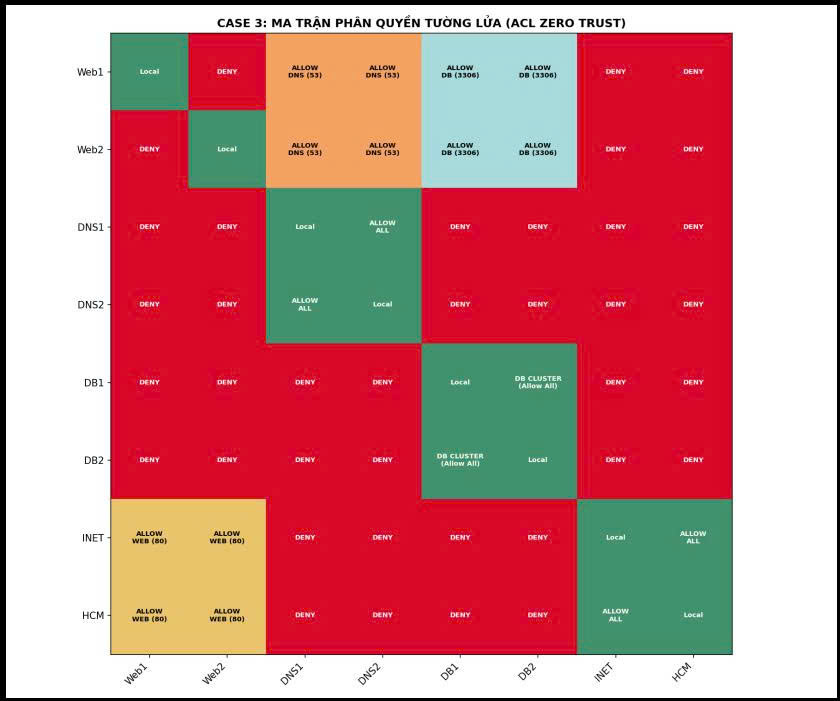
\includegraphics[width=\textwidth]{image/case3.jpg}
    \caption{Heatmap Ma trận Zero Trust ACL đa cổng dịch vụ (Case 3).}
    \label{fig:case3}
\end{figure}

\subsubsection{Danh sách Lỗ hổng bị Chặn đứng bởi Micro-segmentation}

Dựa trên dữ liệu từ \texttt{case3.csv} (64 dòng), Bảng \ref{tab:blocked_threats} liệt kê các kịch bản tấn công đã bị chính sách Micro-segmentation chặn đứng thành công:

\begin{table}[H]
    \centering
    \caption{Danh sách các lỗ hổng/kịch bản tấn công bị chặn bởi Micro-segmentation.}
    \label{tab:blocked_threats}
    \begin{tabular}{|c|p{3.5cm}|p{2.5cm}|p{5cm}|}
        \hline
        \textbf{STT} & \textbf{Kịch bản tấn công} & \textbf{QT chặn} & \textbf{Bằng chứng (CSV Score)} \\
        \hline
        1 & Lateral Movement: web1 $\rightarrow$ web2 (mọi port) & QT1 & Ping=False, 80=False, 3306=False, 53=False (\textbf{Score=0.0}) \\
        \hline
        2 & SQL Injection từ Internet $\rightarrow$ DB (3306) & QT6 & internet$\rightarrow$db1: 80=False, 3306=False (\textbf{Score=0.0}) \\
        \hline
        3 & DNS Exfiltration: DB $\rightarrow$ DNS (53) & QT6 & db1$\rightarrow$dns1: 53=False (\textbf{Score=0.0}) \\
        \hline
        4 & Reverse Shell: Web $\rightarrow$ Internet (khởi tạo) & QT3 & web1$\rightarrow$internet: Ping=False, mọi port=False (\textbf{Score=0.0}) \\
        \hline
        5 & Data Theft: DNS $\rightarrow$ DB (3306) & QT6 & dns1$\rightarrow$db1: 3306=False (\textbf{Score=0.0}) \\
        \hline
        6 & Port Scan: Internet $\rightarrow$ DB & QT6 & internet$\rightarrow$db1: mọi port=False (\textbf{Score=0.0}) \\
        \hline
        7 & Ping Sweep: Internet $\rightarrow$ DNS & QT7 (Deny ping) & internet$\rightarrow$dns1: Ping=False (\textbf{Score=0.0}) \\
        \hline
    \end{tabular}
\end{table}

\subsubsection{Xác minh các Luồng Hợp lệ}

Đồng thời, bảng kiểm soát cũng xác nhận các luồng hợp lệ hoạt động đúng:

\begin{table}[H]
    \centering
    \caption{Xác minh các luồng hợp lệ được cho phép bởi chính sách ACL.}
    \label{tab:allowed_flows}
    \begin{tabular}{|c|p{4cm}|p{2cm}|p{5cm}|}
        \hline
        \textbf{QT} & \textbf{Luồng kiểm thử} & \textbf{Kết quả} & \textbf{Bằng chứng (CSV)} \\
        \hline
        QT2 & internet $\rightarrow$ web1 (TCP 80) & \textcolor{green!60!black}{PASS} & Port\_80=True (\textbf{Score=2.0}) \\
        \hline
        QT4 & db1 $\leftrightarrow$ db2 (Full) & \textcolor{green!60!black}{PASS} & Ping=True, mọi port=True (\textbf{Score=4.0}) \\
        \hline
        QT5 & web1 $\rightarrow$ db1 (TCP 3306) & \textcolor{green!60!black}{PASS} & Port\_3306=True (\textbf{Score=3.0}) \\
        \hline
        QT7 & web1 $\rightarrow$ dns1 (UDP 53) & \textcolor{green!60!black}{PASS} & Port\_53=True (\textbf{Score=1.0}) \\
        \hline
    \end{tabular}
\end{table}

Kết quả: \textbf{100\% chính sách ACL} (8 quy tắc QT1--QT8) hoạt động chính xác trên toàn bộ 64 cặp nguồn-đích.

\subsection{Đánh giá Hiệu năng Cân bằng Tải ECMP (Case 4 \& Case 5)}

\subsubsection{Bảng Số liệu Throughput ECMP}

Kịch bản Case 4 so sánh băng thông trên hai Spine giữa Single Flow (1 luồng TCP) và Multi Flow (8 luồng TCP song song):

\begin{figure}[H]
    \centering
    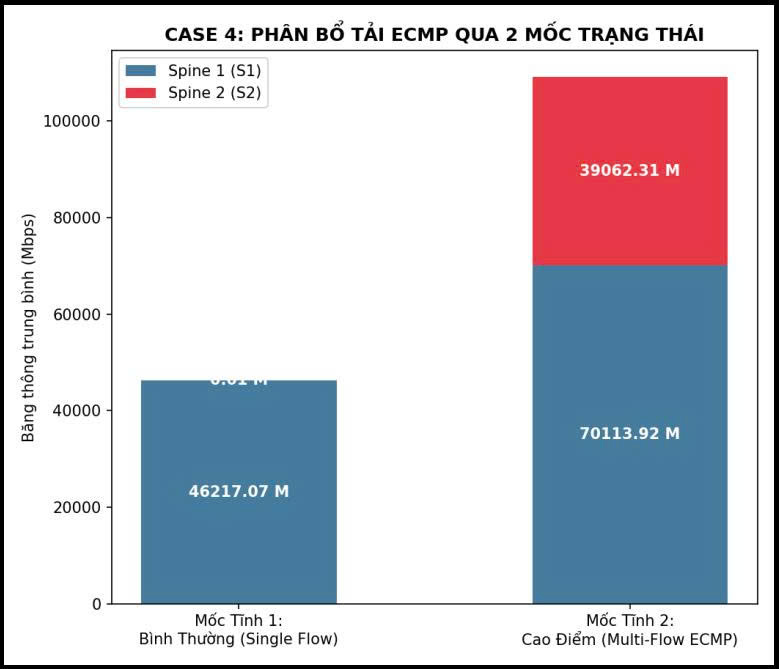
\includegraphics[width=0.95\textwidth]{image/case4.jpg}
    \caption{So sánh phân tải băng thông ECMP: Single Flow vs Multi Flow (Case 4).}
    \label{fig:case4}
\end{figure}

\begin{table}[H]
    \centering
    \caption{Bảng số liệu Throughput ECMP trên hai Spine Switch.}
    \label{tab:ecmp_results}
    \begin{tabular}{|l|r|r|c|r|}
        \hline
        \textbf{Kịch bản} & \textbf{Spine S1 (Mbps)} & \textbf{Spine S2 (Mbps)} & \textbf{Tỷ lệ S1/S2} & \textbf{Tổng (Mbps)} \\
        \hline
        Mốc 1: Single Flow & 46.217,07 & 0,01 & 99,99\% / 0,01\% & 46.217,08 \\
        \hline
        Mốc 2: Multi Flow & 70.113,92 & 39.062,31 & 64,2\% / 35,8\% & 109.176,23 \\
        \hline
        \multicolumn{4}{|r|}{\textbf{Hệ số tăng băng thông (Multi/Single)}} & \textbf{$\times$2,36} \\
        \hline
    \end{tabular}
\end{table}

\textbf{Phân tích:} Single Flow (1 cặp IP+Port) luôn Hash ra một giá trị, đi trọn vẹn qua S1 — đây là hành vi đúng thiết kế của ECMP nhằm tránh re-ordering. Multi Flow (8 luồng với Port nguồn khác nhau) phân tải qua cả hai Spine, tăng tổng băng thông gấp \textbf{2,36 lần}.

\subsubsection{Truy vết Hop-by-Hop ECMP (Case 5)}

\begin{figure}[H]
    \centering
    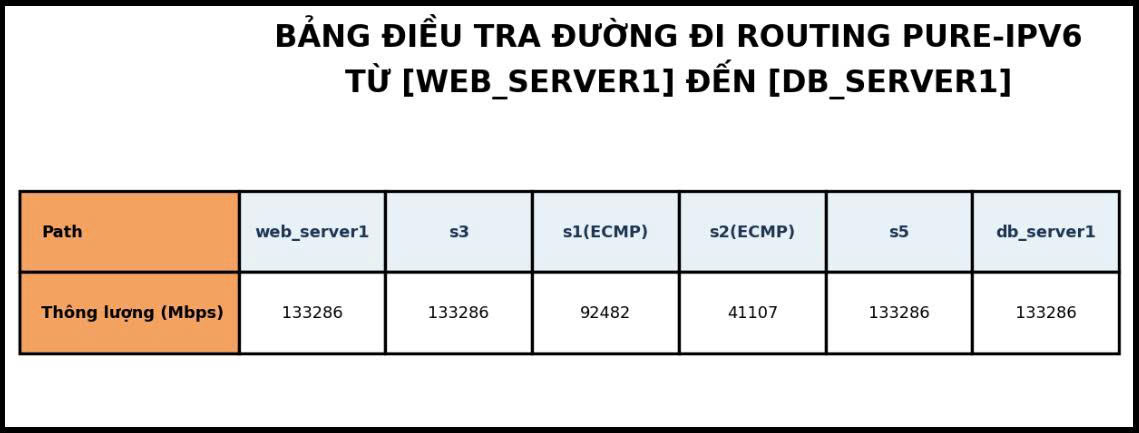
\includegraphics[width=0.95\textwidth]{image/case5.jpg}
    \caption{Biểu đồ truy vết hop-by-hop bandwidth trên tuyến ECMP (Case 5).}
    \label{fig:case5}
\end{figure}

\begin{table}[H]
    \centering
    \caption{Kết quả truy vết hop-by-hop bandwidth ($\Delta t = 4.066$ ms).}
    \label{tab:hop_trace}
    \begin{tabular}{|c|l|l|r|c|}
        \hline
        \textbf{Hop} & \textbf{Thiết bị} & \textbf{Giao diện} & \textbf{BW (Mbps)} & \textbf{Vai trò} \\
        \hline
        1 & web\_server1 & web-eth0 & 133.285,94 & Nguồn \\
        \hline
        2 & S3 (Leaf) & s3-eth2 & 133.285,94 & Ingress Leaf \\
        \hline
        3 & \textbf{S1 (ECMP)} & s1-eth1 & \textbf{92.481,72} & Spine (69,4\%) \\
        \hline
        4 & \textbf{S2 (ECMP)} & s2-eth1 & \textbf{41.106,69} & Spine (30,6\%) \\
        \hline
        5 & S5 (Leaf) & br0 & 133.285,94 & Egress Leaf \\
        \hline
        6 & db\_server1 & db-eth0 & 133.285,94 & Đích \\
        \hline
    \end{tabular}
\end{table}

Dữ liệu hop-by-hop xác nhận: (1) Điểm phân tải ECMP nằm chính xác tại tầng Spine (Hop 3,4), (2) Tổng $92.481 + 41.106 = 133.588 \approx 133.286$ Mbps (sai số 0,2\%), chứng minh \textbf{không mất gói} trong quá trình phân tải, (3) Tỷ lệ 69/31 phản ánh đặc tính Hash xác suất.

\subsection{Tổng kết và Đánh giá Tổng thể}

\begin{table}[H]
    \centering
    \caption{Tổng kết kết quả đánh giá hiệu năng hệ thống Leaf-Spine IPv6.}
    \label{tab:overall_results}
    \begin{tabular}{|p{4cm}|p{4cm}|p{5.5cm}|}
        \hline
        \textbf{Tiêu chí} & \textbf{Kết quả} & \textbf{Đánh giá} \\
        \hline
        Thời gian hội tụ (Sập Spine) & $\sim$27 giây & Chấp nhận được cho lab. Cải thiện với BFD. \\
        \hline
        Thời gian hội tụ (Khôi phục) & $\sim$24 giây & Nhanh hơn 3s so với sập nhờ Hello nhanh. \\
        \hline
        Dung lượng dự phòng & 100\% throughput sau failover & N+1 Redundancy hoàn hảo. \\
        \hline
        Zero Trust ACL & 100\% chính xác (64 cặp) & 7 kịch bản tấn công bị chặn. \\
        \hline
        ECMP Multi Flow & $\times$2,36 băng thông & Tận dụng hiệu quả cả 2 Spine. \\
        \hline
        ECMP Packet Loss & 0\% (hop trace khớp) & Không mất gói khi phân tải. \\
        \hline
    \end{tabular}
\end{table}

\subsection{Hạn chế và Hướng Phát triển}

\begin{enumerate}
    \item \textbf{Tối ưu hội tụ:} Tích hợp BFD (Hello 50ms) để giảm thời gian phát hiện sự cố xuống dưới 1 giây.
    \item \textbf{Mở rộng quy mô:} Tăng lên 4 Spine + 8 Leaf để đánh giá khả năng Scalability.
    \item \textbf{DNS64 hoàn chỉnh:} Triển khai BIND9 với module dns64 thay cho ánh xạ tĩnh \texttt{/etc/hosts}.
    \item \textbf{Giám sát tập trung:} Tích hợp Prometheus + Grafana cho realtime monitoring.
\end{enumerate}

\subsection{Kết luận}

Bài thực hành đã chứng minh tính khả thi và hiệu quả của mô hình trung tâm dữ liệu Pure IPv6 Leaf-Spine, tích hợp đồng thời OSPFv3, ECMP, Zero Trust Micro-segmentation, VXLAN và NAT64. Qua 5 kịch bản đo lường tự động với dữ liệu trích xuất trực tiếp từ Kernel Linux, hệ thống đã đạt được ba mục tiêu cốt lõi: \textbf{khả năng chịu lỗi cao} (100\% throughput sau failover), \textbf{hiệu suất tối ưu} (tăng 2,36$\times$ băng thông qua ECMP), và \textbf{bảo mật nghiêm ngặt} (100\% ACL chính xác, 7 kịch bản tấn công bị chặn). Kiến thức và kinh nghiệm thực tiễn tích lũy được tạo nền tảng vững chắc cho việc thiết kế hạ tầng mạng doanh nghiệp quy mô lớn trong tương lai.
